\setlength\epigraphwidth{9cm}
\epigraph{[The formalism of quantum mechanics] is a peculiar mixture describing in part realities of Nature, in part incomplete human information about Nature -- all scrambled up by Heisenberg and Bohr into an omelette that nobody has seen how to unscramble.}{--- Edwin T. Jaynes}
% "Probability in Quantum Theory" in Complexity, Entropy, and the Physics of Information, W. H. Zurek (ed.), Addison-Wesley, Redwood City, CA, p. 381

%------------------------------------
%\section{็Quantum theory in phase space}
%------------------------------------

Just as classical mechanics can be formulated in many different ways---Newtonian, Lagrangian, Hamiltonian, to give some examples---so, too, can quantum mechanics~\cite{styer2002nine}.  Different formulations bring to the fore different aspects of the theory even as they obscure others. The focus of this dissertation is on the phase space formulations of quantum theory, in which the usual complex Hilbert space retreats into the background, and a picture resembling that of classical statistical mechanics emerges.

The concept of a phase space has its roots in classical Hamiltonian mechanics. It gives a complete description of a system in terms of conjugate variables, $\{q_j\}$ and $\{p_j\}$, defined by the Poisson bracket
\begin{align}
\{ q_j,p_k \}_{PB} = \delta_{jk},
\end{align}
where
\begin{align}
	\{ f,g \}_{PB} &= \sum_j \frac{\partial f}{\partial q_j} \frac{\partial g}{\partial p_j} - \frac{\partial g}{\partial q_j} \frac{\partial f}{\partial p_j}.
\end{align}
The word ``phase" in ``phase space" originated from Boltzmann when he described instantaneous points in the Lissajous pattern of two harmonic oscillators by their instantaneous relative phase. The trajectory of these \emph{phase points} fills the entire space bounded by the oscillators' amplitudes when the ratio of the frequencies of the two oscillators is irrational, a circumstance which would later become Boltzmann's ergodic hypothesis \cite{nolte_tangled_2010}.

The Heisenberg uncertainty relation prevents a deterministic phase space description of a quantum system completely localized in both of its conjugate variables, such as position and momentum---there are no quantum phase points!
This does not, however, prevent a statistical formulation of quantum theory on a phase space. The first example was developed by Wigner, who showed that quantum expectation values can be calculated as averages over phase space distributions, now known as \emph{Wigner functions} \cite{wigner_quantum_1932}. Wigner functions are not true probability densities and are said to be \emph{quasi-probabilities} as they take on negative values for some states. Moyal \cite{moyal_quantum_1949} noticed that Wigner's quasi-probability map is the inverse of Weyl's quantization rule that maps distributions to quantum operators \cite{weyl_quantenmechanik_1927}. Independently, Moyal and Groenewold \cite{groenewold_principles_1946} established the Wigner-Weyl phase space picture as an autonomous formulation of quantum mechanics. (For the interested reader, historically important papers, each accompanied by a brief annotation, are collected in \cite{zachos2005quantum}.) 

The notion of a Wigner function, which to many is synonym to that of a quasi-probability representation, has been generalized to physical systems with other symmetries, for example, the Poincar{\'e} symmetry of special relativity~\cite{kim1991phase,schroeck1996quantum}. The spherical phase space representation \cite{stratonovich_distributions_1957} and discrete phase spaces---the one by Hannay and Berry \cite{hannay_quantization_1980} being the first that appeared in the literature---are one of the many generalizations \cite{ferrie_quasi-probability_2011} of the Wigner function to finite-dimensional (spin) systems.

%The phase space representation is by now an essential tool in the field of quantum optics \cite{cahill_density_1969,sudarshan_equivalence_1963,hillery_distribution_1984,lee_theory_1995}.

 %Ones of the most popular quasi-probability representations of quantum theory such as the Galuber-Sudarshan P \cite{cahill_density_1969,sudarshan_equivalence_1963} and Husimi Q \cite{husimi_formal_1940} distributions share the same phase space $\mathbb{R}^{2n}$ with the Wigner function, and there are many discretized variants of the phase space.

There is a tendency to associate negativity of quasi-probability distributions with non-classicality of quantum states. In the Glauber-Sudarshan \emph{P representation} \cite{glauber_coherent_1963, sudarshan_equivalence_1963}, the only states that make $P$ a true probability distribution are mixtures (convex combinations) of coherent states $\{\ket{\alpha}\}$. Introduced by Schr{\"o}dinger as ``the most classical" states of a harmonic oscillator, coherent states are states with minimal uncertainty, equally distributed between the two quadratures. Glauber coined the term ``coherent states" and ascribed them to quantum states of light that can be modeled by a stochastic classical electromagnetic field. Non-coherent states such as squeezed states and photon number states have negative $P$ distributions and are often thought of as non-classical states. %Squeezed states have negative P distributions and can offer better sensitivity over classical light in some metrological tasks \cite{walls2007quantum}.
The difficulty in associating negativity and non-classicality is that the choice of the quasi-probability representation is not unique. A state with a negative quasi-probability distribution in one representation may have a positive quasi-probability distribution in another representation. For instance, the Wigner functions of all Gaussian states including the squeezed ones are non-negative. In fact, in the Husimi $Q$ representation \cite{husimi_formal_1940}:
\begin{align}
	Q_{\rho}(\alpha) &= \braket{\alpha| \rho |\alpha}
\end{align}
every state has a positive distribution. So negativity of a quasi-probability distribution \emph{per se} cannot be an indicator of non-classicality. An operational approach can offer a resolution to this difficulty. What we can do with a quantum state depends on which measurements we are allowed to make, and vice versa. So an operationally motivated definition of non-classicality must consider both states and measurements in conjunction.

Once the full quantum formalism is taken into account, does there exist a quasi-probability representation that displays no negativity at all? Intuitively, this cannot be the case because otherwise quantum theory would be reduced to a classical statistical theory. Indeed, the answer for finite dimensions was given in the negative, independently in \cite{spekkens_negativity_2008} and \cite{ferrie_frame_2008,ferrie_framed_2009}, while \cite{ferrie_necessity_2010} generalizes the latter proof to infinite dimensional Hilbert spaces. Thus, the problem shifts to finding a \emph{non-negative subtheory}: a subset of quantum states and measurements that are represented by non-negative quasi-probability distributions \cite{wallman_non-negative_2012}. A phase space representation automatically supplies a classical statistical theory, a hidden variable theory (a non-contextual hidden variable theory in the sense of Spekkens \cite{spekkens_negativity_2008} to be exact, since a quasi-probability mapping of an operator is defined to be one-one) for the non-negative subtheory in that representation (if exists). Thus, a phase space representation suggests a natural boundary between what is classical and what is intrinsically quantum.

Fast-forwarding to the present, an interest in non-negative subtheories has been renewed by the possibility of a quantum computer, a machine that makes use of fragile quantum effects which typically do not survive in an uncontrolled en\-vi\-ron\-ment, to solve particular problems faster than any known classical method. For simplicity, what we mean by a quantum computer is a \emph{universal} one that can simulate any quantum computer with at most a resource that is polynomial in the size $n$ of the input, or more precisely $\mathcal{O}(n^k)$ for some positive number $k$. We write $f(n)=\mathcal{O}(g(n))$ and say that the function $f(n)$ grows as $g(n)$ if there is a positive constant $c$ such that, for some $n_0$,
\begin{align}
	|f(n)| \le c|g(n)|,
\end{align}
when $n>n_0$, that is, asymptotically. Polynomial functions are closed in the sense that a composition of polynomials is also a polynomial. So in a very coarse-grained point of view, if we deem algorithms that run in time proportional to the input size ($f(n) = n$) efficient, then it is natural to call a concatenation of these linear-time algorithms efficient as well. Admittedly, the degree of the polynomial can be very high, but phenomenologically this notion of efficiency seems to be robust, as most polynomial-time algorithms turn out to be practical \cite{AB,aaronson2013democritus}.

\begin{figure}[H]
	\begin{center}
		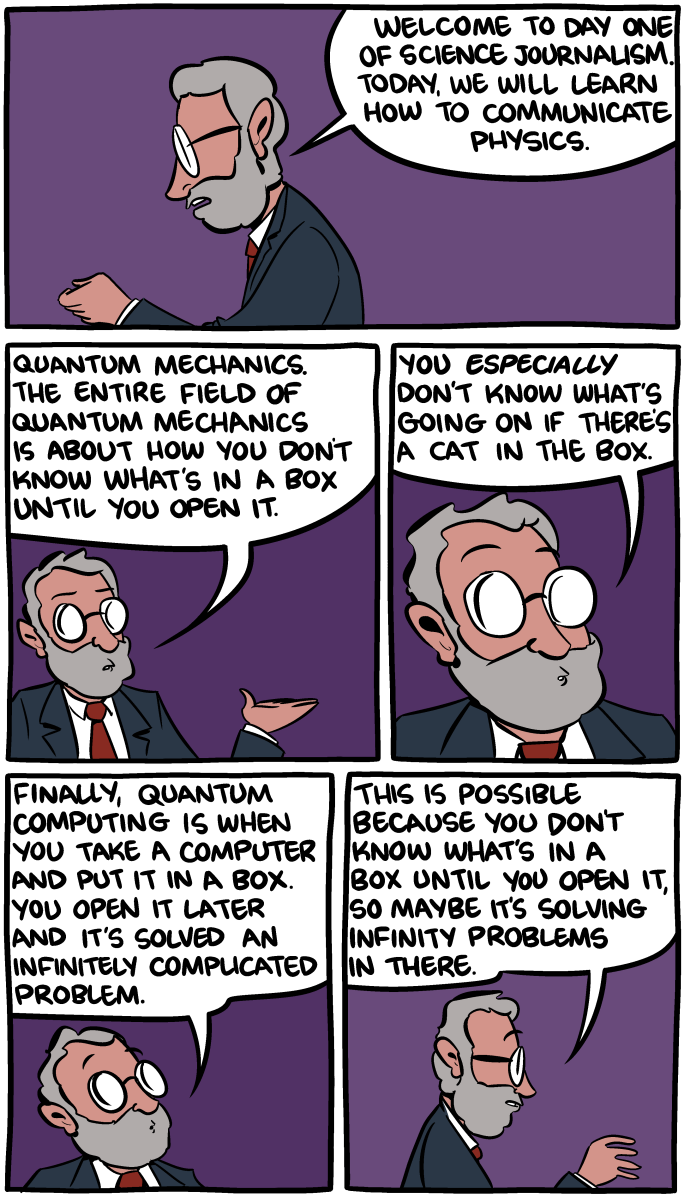
\includegraphics[width=0.5\textwidth]{img/smbc-science-communication.png}
			\caption{In a quantum world, a cat can be dead or alive; knowing that an electron here is in the ``spin up" state instantaneously collapses an electron on the other side of the universe to the ``spin down" state.
			Prompted by this description of the quantum world, an intelligent seven-year-old might say: ``What's the big deal? The cat is either alive or dead. We just couldn't tell until we look at it. Also, the pair of electrons is no different from a pair of gloves. If I know that one of the gloves is left handed, the other one must be right handed."
			And the kid would be right! Classical randomness and classical correlation suffice to explain any outcome of a quantum measurement done in a single fixed basis.
			(The comic is reprinted with permission from the author \cite{SMBC}.)}
			\label{fig:smbc-comics}
	\end{center}
\end{figure}

With a growing list of problems that are easier to solve on a quantum computer than a classical one \cite{jordan2017zoo}, it is natural to ask: where does the quantum speed-up come from?  For concreteness, let us assume that our quantum computer is composed of $n$ qubits i.e. spin-1/2 systems in pure states.  What a quantum computer of this sort does is nothing but rotating a $2^n$-dimensional complex vector around.  Thus we might look for a physical system with a similar mathematical structure and see why we cannot use it to achieve the same effect as quantum speed-up. For example, classical waves are also described by complex amplitudes. So why can't we let classical waves perform quantum computation? The problem is that the number of modes needed to simulate the Hilbert space of $n$ qubits scales exponentially in $n$ because classical waves lack the entanglement that makes up the exponentially large composite Hilbert space \cite{jozsa1997entanglement,blume-kohout_climbing_2002}.

%Classical waves can superpose but the number of modes needed to simulate the Hilbert space scales exponentially because they lack the tensor product structure ---that is, entanglement-- that makes up an exponentially large composite Hilbert space \cite{jozsa1997entanglement,blume-kohout_climbing_2002}. Soon after it was shown that entanglement, quantified by a suitable entanglement measure, is necessary to achieve an exponential speed-up in pure state quantum computation \cite{jozsa_role_2003,vidal_efficient_2003}. \cite{van_den_nest_universal_2013} showed that quantum computation with little entanglement according to continuous entanglement measures can still perform a universal quantum computation. Moreover, quantum computers are able to explore only a little corner of the exponentially large Hilbert space in a polynomial time \cite{poulin_quantum_2011}. The source of a quantum computer's efficiency may remains illusive in the most general setting \cite{vedral_elusive_2010}.

Insight can be gained by comparing quantum and probabilistic computations. Suppose that a coin flip has the probability $p$ of coming up heads and $q=1-p$ of coming up tails. The joint probability vector of outcomes of flipping $n$ independent coins is the tensor product of the probability vector of outcomes of each coin flip. For two coins, for example,
\begin{align}
	\begin{pmatrix}
		p_1 \\ q_1
	\end{pmatrix}
	\otimes
	\begin{pmatrix}
		p_2 \\ q_2
	\end{pmatrix}
	&=
	\begin{pmatrix}
		p_1 p_2 \\
		p_1 q_2 \\
		q_1 p_2 \\
		q_1 q_2
	\end{pmatrix}.
\end{align}
We see that the process of flipping $n$ coins also happens in an exponentially large vector space. Thus, the size of the Hilbert space cannot be the explanation of quantum speed-up \emph{per se}.\footnote{Also, quantum computers are only capable of exploring an exponentially small corner of the Hilbert space in polynomial time \cite{poulin_quantum_2011}.} To further amplify the similarity, the complex amplitudes can be replaced by real amplitudes without compromising the computing power \cite{bernstein_quantum_1997,adleman_quantum_1997,rudolph_2_2002,aharonov_simple_2003}. This leaves us with two differences: quantum amplitudes can take negative values, and quantum probabilities
are 2-norms instead of 1-norms. From this perspective, negative amplitudes are important because they allow \emph{destructive interference}: different computational paths that lead to the same configuration can cancel each other. (This viewpoint is popularized by Scott Aaronson in his lecture-turned-book, \emph{Quantum Computing Since Democritus} \cite{aaronson2013democritus}.) The reader who still remembers the main topic of the dissertation might see where this story is going. We can go further and turn quantum computation into probabilistic computation with \emph{negative} probabilities, as did Feynman more than 30 years ago \cite{feynman_simulating_1982}. He introduced a quasi-probability representation for a qubit identical to that of Wootters \cite{wootters_wigner-function_1987} and observed that
\begin{quote}
The only difference between a probabilistic classical world and the equations of the quantum world is that somehow or other it appears as if the probabilities would have to go negative, and that we do not know, as far as I know, how to [efficiently] simulate.
\end{quote}
Nonetheless, whenever the quasi-probability is amenable to an efficient sampling throughout the computation, one adds to the repertoire statistical techniques such as Monte Carlo methods to simulate quantum computation.

Over the years, several results have shown that pure state quantum computation with little entanglement (quantified by a discrete entanglement measure such as the Schmidt rank \cite{van_den_nest_universal_2013}) can be efficiently simulated classically; references \cite{jozsa_role_2003,vidal_efficient_2003,yoran_classical_2006,jozsa_simulation_2006} work in the unitary-gate model while references \cite{markov_simulating_2008,shi_classical_2006,van_den_nest_classical_2007} work in the measurement-based model. However, it can be argued that while entanglement is necessary in these models, it is not sufficient. The Gottesman-Knill theorem provides an efficient classical simulation of any stabilizer computation \cite{gottesman_stabilizer_1997,nielsen2000quantum}; such computations generate states called stabilizer states, which can be highly entangled, an example being the GHZ state $(\ket{0}^{\otimes n} + \ket{1}^{\otimes n})/\sqrt2$. Stabilizer computation can be recast not only as (a subset of) probabilistic computation embedded in quantum computation\footnote{The embedding is the following standard one: probabilistic computation is equivalent to quantum computation using only gates diagonal in the computation basis, supplemented by Hadamard gates to simulate coin flips \cite{nielsen2000quantum}.} \cite{nest_classical_2008}, explaining its ``weak" computational power, but also as a non-negative subtheory---at least half the time. Stabilizer computation and the Gottesman-Knill theorem can be generalized from two-level systems to $d$-level systems \cite{gottesman_fault-tolerant_1999}. In \cite{gross_hudsons_2006}, Gross found that only in odd dimensions does there exist a unique discrete analogue of the Wigner representation in which a pure state has a non-negative Wigner function if and only if it is a  stabilizer state, thus proving the discrete version of the Hudson's theorem that the only continuous-variable pure states with non-negative Wigner functions are Gaussians \cite{hudson_when_1974}. This raises the question of the positivity of the discrete Wigner functions of mixed states. The fact that there are mixed states outside the convex hull of stabilizer states with positive discrete Wigner functions allows generalizations of the odd-dimensional Gottesman-Knill theorem \cite{mari_positive_2012,veitch_negative_2012}. In the continuous-variable case, references \cite{srinivas_nonclassical_1975,brocker_mixed_1995} found that a theorem in classical probability attributed to Bochner \cite{bochner_monotone_1933} and generalizations thereof can be used to characterize both the valid Wigner functions and the subset of positive ones. This motivates us to look for a quantum version of Bochner's theorem in discrete phase spaces reported in Chapter \ref{ch:commutative-phase-space}.

An efficiently simulatable subtheory and a non-negative subtheory are related but distinct concepts. An arbitrary probability distribution may not be amenable to an efficient sampling scheme. For this reason, the input state in \cite{mari_positive_2012,veitch_negative_2012} is restricted to be a product state. However, as pointed out in the papers, any quasi-probability function that can be sampled efficiently allows a classical simulation. Conversely, outcome probabilities from negative quasi-probability functions can be estimated at a cost exponential in the total negativity of states, operations, or measurements \cite{pashayan_estimating_2015}, but still allowing estimation of an outcome of a quantum computation with polynomially growing negativity.

%\emph{Stabilizer states} were originally defined for multiple qubits \cite{gottesman_stabilizer_1997} and have a plethora of applications in quantum error correction and quantum computation \cite{fujii2015quantum}.
%In odd dimensions, they have the following equivalent characterizations:
%\begin{enumerate}
%	
%	\item\label{def-stabilizer} Each stabilizer state is a joint eigenvector of a \emph{stabilizer subgroup} -- a maximal abelian subgroup of the generalized Pauli group $\mathcal{P}_d$.
%	
%	\item\label{clifford-orbit} Stabilizer states are the orbit of the state $\ket{0}$ under the Clifford group.
%	
%	\item\label{gaussian-wave-function} Their wave functions have a Gaussian form in the standard basis $\{\ket{m}| m=0,\dots, d-1 \}$
%	\begin{align}
%	\psi(m) = \omega^{mAm + bm},
%	\end{align}
%	where $A$ is a symmetric matrix with entries in $\mathbb{Z}_d$ and $b \in \mathbb{Z}^d$.	
%	
%\end{enumerate}
%Especially properties \ref{clifford-orbit} and \ref{gaussian-wave-function} affirm the status of stabilizer states as the natural discrete analogue of Gaussian states.
%
%The analogy between stabilizer and Gaussian states can be pursuit further. The \emph{stabilizer subtheory} -- the operational subtheory of quantum theory consisting of all stabilizer state preparations and generalized Pauli measurements (and implicitly Clifford transformations) -- is extremely unusual and interesting.\footnote{An ontological model ``close" to the stabilizer subtheory can be defined and studied for even-dimensional classical dits but there is no corresponding subtheory of quantum theory \cite{spekkens_evidence_2007,pusey_stabilizer_2012,catani_spekkens_2017}.} On the one hand, it displays features that many would deem exclusively quantum such as superposition and teleportation. It contains highly entangled states such as the GHZ state $d^{-n/2} \sum_{m=0}^{d-1} \ket{m}^{\otimes n}$. On the other hand, the subtheory is classical in both of the following senses:
%\begin{enumerate}
%	
%	\item its states and probabilities of obtaining a given measurement outcome are efficiently classically simulatable by the \emph{Gottesman-Knill theorem} \cite{nielsen2000quantum,aaronson_improved_2004}.
%	
%	\item By the discrete Hudson's theorem, it has as an ontological model the discrete Wigner phase space.
%\end{enumerate}
%One can readily compare the stabilizer subtheory to the classically efficiently simulatable \emph{Gaussian subtheory} -- the operational subtheory of quantum theory consisting of preparations of Gaussian states and Gaussian measurements (such as homodyne and heterodyne measurements) \cite{bartlett_efficient_2002}.

Another well-known efficiently simulatable subtheory is matchgate computation. While the stabilizer model of computation requires that the gates are implemented only in discrete time steps, matchgates are more ``physical" in the sense that they form a continuous set of gates infinitesimally generated by Hamiltonians. Matchgates were introduced by Valiant \cite{valiant_quantum_2002,valiant_holographic_2008} in the context of algorithms for graphs and have several interesting properties. For example, the power of matchgate computation depends strongly on the connectivity of matchgate interaction. In the spin-1/2 model, the anisotropic Heisenberg interaction,
\begin{align}
	H_H &= X_jX_k + Y_jY_k,
\end{align}
where $X$ and $Y$ are Pauli matrices,
generates matchgates and is capable of universal quantum computation if the interaction is not limited to only nearest neighbor (N.N) spins \cite{divincenzo_universal_2000,kempe_encoded_2001,kempe_exact_2002}. It turns out that N.N. matchgate computation is classical simulatable and just the addition of next-nearest-neighbor matchgates or equivalently the swap operation
\begin{align}
	\begin{pmatrix}
		1 & 0 & 0 & 0 \\
		0 & 0 & 1 & 0 \\
		0 & 1 & 0 & 0 \\
		0 & 0 & 0 & 1
	\end{pmatrix},
\end{align}
itself not a matchgate, promotes N.N. matchgates to universality \cite{jozsa_matchgates_2008}. N.N. matchgate computation is also equivalent, via the Jordan-Wigner transformation, to the evolution of a system of non-interacting fermions---so-called fermionic linear optics \cite{knill_fermionic_2001,terhal_classical_2002}.

The obvious question (also raised in \cite{brod_efficient_2016}) is whether fermionic linear optics can be formulated as a non-negative subtheory, and if not, can we find a quasi-probability representation in which the negativity of the classically simulatable states and measurements only grows polynomially? Given an infinitude of possible quasi-probability representations, a sensible starting point is to impose symmetry. The classical simulations of stabilizer computation and bosonic linear optics (including squeezing) in \cite{veitch_negative_2012,veitch_efficient_2013} are facilitated by the fact that the (discrete and continuous) Wigner function is \emph{covariant} with respect to the (discrete and continuous, respectively) affine symplectic group. 

A group $G$, generally, plays double role in a $G$-covariant phase space representation; it acts on a quantum operator $A$ through a unitary representation $U(g)$ on the Hilbert space
\begin{align}
	A &\mapsto U\dgg(g) A U(g),
\end{align}
where $g \in G$, and it acts on the phase space by permutations of phase points. In particular, operators that lie in the same orbit of the group exhibit the same amount of negativity in their quasi-probability distributions. $G$-covariance is thus a quite natural constraint if one wants to interpret negativity as non-classicality and has a reason that $G$ should be thought of as a classical dynamics. %For fermionic linear optics, the classical dynamics is the orthogonal group $\gr{SO}{2n}$, where $n$ is the number of modes or qubits.

A simple way to obtain a $G$-covariant quasi-probability function is to pick a fiducial state $\ket{e}$ in the Hilbert space, a computational basis state $\ket{0 0 \cdots 0 }$ for instance, and generate the orbit under $G$:
\begin{align}
	\ket{\Omega} &= U(\Omega) \ket{e},
\end{align}
where $U(\Omega)$ is an equivalence class of $\{ U(g)\}$ that give the same state $\ket{\Omega}$ up to a phase. By identifying $\{\Omega\}$ with phase points, the analogue of the $Q$ function
\begin{align}
	\mu_{\rho}(\Omega) &= \braket{\Omega|\rho|\Omega}.
\end{align}
is guaranteed to be $G$-covariant. For our purpose though, the function is not very interesting because it is non-negative everywhere.\footnote{This is the spirit of the approach taken by Drummond \emph{et al.} to write down a Fokker-Planck-type equation that describes fermionic dynamics \cite{corney_gaussian_2006,corney_gaussian_2006-1,rosales-zarate_probabilistic_2015}.} Building from this idea, Brif and Mann \cite{brif_phase-space_1999} devised a general construction of $G$-covariant phase spaces for any Lie group $G$, obeying the \emph{Stratonovich-Weyl correspondence} attributed to \cite{stratonovich_distributions_1957}. Mathematical physicists are particularly interested in the correspondence since it gives rise to interesting new quantization maps (some of which are mentioned in \cite{brif_phase-space_1999}). Recent years have also seen a renewed interest in $\gr{SU}{n}$-covariant quasi-probability representations for the purpose of visualization, state estimation, and entanglement detection \cite{klimov_general_2010,tilma_sun-symmetric_2012,rios_symbol_2014,tilma_wigner_2016,rundle_simple_2017}. What sets our work apart from these investigations is that we are not interested in the full unitary dynamics $\gr{SU}{2^n}$ on the exponentially large Hilbert space. Instead we are interested in a much smaller set of ``classical", restricted dynamics, namely $\gr{SO}{2n} \subset \gr{SU}{2^n}$.

%------------------------------------
%\section{็When in doubt, make the symmetry counts!}
%------------------------------------

%------------------------------------
%\section{็Dissertation Outline}
%------------------------------------

In Chapter \ref{ch:rep}, we give an overview of the mathematical machineries that we will need later under the umbrella subject of representation theory, with the main goal to develop  harmonic analysis and the notion of spherical functions on our phase spaces, which are compact, multiplicity-free spaces based on semisimple Lie groups.
Chapter \ref{ch:quasi-rep} formally introduces quasi-probability representations in the most general setting, and reviews the proof \cite{ferrie_frame_2008} of the impossibility of a non-negative representation of the full quantum formalism. We then focus on $G$-covariant phase space representations and ones that satisfy the Stratonovich-Weyl correspondence, called \emph{SW representations} for short. Utilizing tools from Chapter \ref{ch:rep}, we provide a slightly different, more algebraic approach to the construction of SW representations than the one presented in \cite{brif_phase-space_1999}. Along the way, we show that, with an additional mild differentiability assumption, the SW representations constructed are essentially unique. Thus, any alternative of the $\gr{SO}{2n}$-covariant phase space representations for fermions in Chapter \ref{ch:matchgate} must violate at least one of our assumptions.

In Chapter \ref{ch:commutative-phase-space}, we review the familiar commutative phase space of Wigner and its not-so-familiar discrete analogue by Gross \cite{gross_hudsons_2006} to prepare the reader for our result. (As a bonus, a cute, short proof by Gross \cite{gross2015coogee} of the discrete Hudson's theorem is provided in full in Appendix \ref{app:hudson}.) We then present a generalization of the quantum Bochner's theorem, applicable to Gross Wigner function and other quasi-probability representations that we construct based on unitary operator bases.

In Chapter~\ref{ch:matchgate}, we take a closer look at matchgates and fermionic linear optics. After a brief discussion of other existing approaches to fermionic phase spaces, we apply our construction of SW representations to fermionic linear optics. The main result is the explicit SW representations in the first non-trivial case: the case of four fermionic modes. The quasi-probability functions of fermionic Gaussian states are found to be negative and the volume of negativity is calculated. (The calculation itself is quite interesting, making use of the fact that our phase space is symmetric and K{\"a}hler (Appendix \ref{app:kahler}).) The last chapter concludes with a summary of results and a dozen open problems pertaining to fermionic phase spaces.

%------------------------------------
%\section{็List of publications and projects}
%------------------------------------

Below are projects that I have completed and have appeared in publication form.
\begin{enumerate}
	\item Ninnat Dangniam and Christopher Ferrie, "Quantum Bochner's theorem for phase spaces built on projective representations," \href{https://doi.org/10.1088/1751-8113/48/11/115305}{\emph{Journal of Physics A: Mathematical and Theoretical} {\bf 11} 115305 (2015)}.
	\item Jonathan A. Gross, Ninnat Dangniam, Christopher Ferrie and Carlton M. Caves, "Novelty, efficacy, and significance of weak measurements for quantum tomography." \href{https://doi.org/10.1103/PhysRevA.92.062133}{\emph{Physical Review A} {\bf 92} 062133 (2015).}
\end{enumerate}
The result in the first paper is described in Chapter \ref{ch:commutative-phase-space}. The new results on Stratonov\-ich-Weyl representations and fermionic phase spaces obtained in collaboration with Christopher Ferrie, Carlton M. Caves and Christopher Jackson will most likely be polished, extended, and submitted for publication in the future.
